\section{Part I: what a memory gap is made of}
\label{sec:results}

All numbers in this section come from the 60 runs of plan \texttt{C08-PARTE1-TALLER} (30 seeds
$\times$ 2 architectures) and their re-evaluations. Unless stated otherwise, intervals are 95\%
percentile bootstrap intervals over seeds (10,000 resamples) and ``pp'' means percentage points.

\subsection{The LSTM outperforms the memory-free MLP on every seed but one}
\label{sec:results-gap}

\Cref{fig:curves} shows the learning curves. Both agents start near the random policy. The MLP
improves steadily but levels off around 50--55\% validation success; the LSTM overtakes it after
about 100,000 interactions and keeps improving to above 80\%. On the test panel
(\cref{tab:summary}) the LSTM reaches 84.0\% final success (SD across seeds 8.7\pp) and the MLP
58.9\% (SD 8.2\pp). The paired gap is $+25.1$\pp{} $[20.8, 29.5]$; the LSTM is ahead on 29 of the
30 seeds and tied on the remaining one (\cref{fig:paired}). None of 200,000 random sign flips of
the paired gaps produced a mean as extreme as the observed one ($p<10^{-5}$). The validation AUC
tells the same story with a smaller gap ($+5.8$\pp{} $[4.0, 7.6]$), because both curves are low
during the first half of training.

By the protocol's acquisition rule, 26 of 30 LSTM runs acquire task~B, at a median of 170,000
interactions (range 130,000--190,000); no MLP run does. Part~I therefore confirms the pilot's
observation with ten times more seeds. It does not say why the LSTM wins: it is also 3.9 times
larger. \Cref{sec:part2} addresses that.

\begin{figure}[t]
  \centering
  \begin{minipage}[t]{0.49\linewidth}
    \centering
    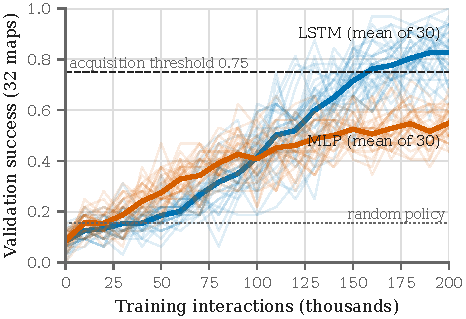
\includegraphics[width=\linewidth]{figures/fig_learning_curves.pdf}
    \caption{Validation success during training (one evaluation per point, 32 maps). Thin
    lines are individual seeds; thick lines are means over 30 seeds.}
    \label{fig:curves}
  \end{minipage}\hfill
  \begin{minipage}[t]{0.49\linewidth}
    \centering
    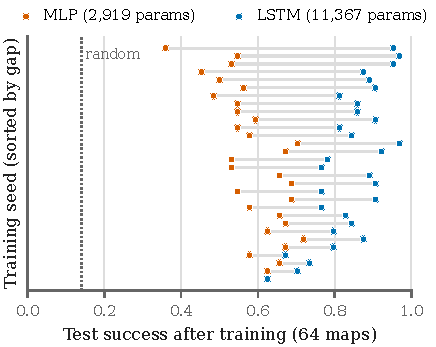
\includegraphics[width=\linewidth]{figures/fig_paired_seeds.pdf}
    \caption{Final test success of each training seed for both architectures, sorted by the
    paired gap. The LSTM is ahead on 29 seeds and tied on one.}
    \label{fig:paired}
  \end{minipage}
\end{figure}

\begin{table}[t]
  \centering
  \caption{Part I summary over 30 paired seeds. Final test success is one evaluation on 64 test
  maps; ``re-evaluated'' averages three further evaluations with new sampling seeds. Brackets
  are 95\% bootstrap intervals over seeds; IQM is the interquartile mean
  \citep{agarwal2021precipice}.}
  \label{tab:summary}
  \small
  \begin{tabular}{lccc}
    \toprule
    & LSTM & MLP & LSTM $-$ MLP (paired) \\
    \midrule
    Trainable parameters & 11,367 & 2,919 & \\
    Final test success (mean) & 84.0 [80.8, 86.9] & 58.9 [55.9, 61.7] & $+25.1$ [20.8, 29.5] \\
    Final test success (IQM) & 84.9 & 59.2 & $+24.3$ \\
    Final test success, re-evaluated & 83.9 [81.0, 86.7] & 58.7 [56.5, 61.0] & \\
    Validation AUC & 44.6 [43.0, 46.1] & 38.8 [37.9, 39.7] & $+5.8$ [4.0, 7.6] \\
    Seeds acquiring B & 26 / 30 & 0 / 30 & \\
    Median acquisition step & 170k & --- & \\
    Test success before training & 11.3 & 12.2 & \\
    \bottomrule
  \end{tabular}
\end{table}

\subsection{Runs are exactly reproducible, and one evaluation is unbiased}
\label{sec:results-repro}

The pilot seeds (7, 19, 31) were run again inside Part~I, now saving a checkpoint at every
evaluation. For all six of them (both architectures) the final weights are identical, bit for
bit, to the pilot's, and so are their test scores. Saving extra checkpoints and re-evaluating
them did not perturb training.

Re-evaluating the final weights three more times leaves the means unchanged (84.0 versus 83.9 for
the LSTM, 58.9 versus 58.7 for the MLP; \cref{tab:summary}): the single evaluation is not biased.
It is, however, noisy. Across seeds, the scores of two re-evaluations of the same weights
correlate at only 0.81 for the LSTM and 0.70 for the MLP.

\subsection{Where the variation comes from}
\label{sec:results-variance}

\Cref{tab:components} gives the variance components of \cref{eq:model} for final test success,
and \cref{fig:composition} turns them into the quantity that matters for a comparison: of the
differences we see between the scores of different seeds, how much is real (seed, and seed
$\times$ map on this panel) and how much is evaluation noise.

For final test success the answer is reassuring. Evaluation noise explains 16\% of the
between-seed variance for the LSTM, 37\% for the MLP and 25\% for the paired gap; most of what
separates seeds is real. Two other metrics behave very differently:
\begin{itemize}
  \item \textbf{Validation AUC of the MLP} is 75\% noise. MLP seeds learn almost identically
  ($\hat\sigma^2_{\text{seed}}\approx 0.0002$), so the little variation there is between them is
  mostly the randomness of 32-map evaluations. The AUC of the \emph{gap}, by contrast, is only
  19\% noise.
  \item \textbf{The acquisition verdict} is 76\% noise. Whether a given LSTM run ``acquired'' the
  task depends mostly on the sampling seeds of its validation episodes: replaying the same
  checkpoints with the three new sampling seeds changes the verdict for 8 of the 30 LSTM runs.
  The component interval is wide ($\sigma^2_{\text{seed}}\in[0, 0.082]$) and includes zero.
\end{itemize}
The map is the largest single component for final test success (\cref{tab:components}). It does
not add uncertainty to a comparison on the fixed test panel, which both architectures share, but
it dominates any claim about maps outside the panel (\cref{sec:results-seeds}).

\begin{table}[t]
  \centering
  \caption{Variance components of final test success per episode (\cref{eq:model}; $S=30$,
  $M=64$, $R=3$), with 95\% seed-bootstrap intervals.}
  \label{tab:components}
  \small
  \begin{tabular}{lccc}
    \toprule
    Component & LSTM & MLP & LSTM $-$ MLP \\
    \midrule
    $\sigma^2_{\text{seed}}$ & 0.0059 [0.0030, 0.0087] & 0.0032 [0.0012, 0.0053] & 0.0096 [0.0043, 0.0151] \\
    $\sigma^2_{\text{map}}$ & 0.0346 [0.0275, 0.0469] & 0.0911 [0.0820, 0.1056] & 0.0368 [0.0332, 0.0486] \\
    $\sigma^2_{\text{seed}\times\text{map}}$ & 0.0174 [0.0104, 0.0210] & 0.0184 [0.0090, 0.0231] & 0.0362 [0.0191, 0.0461] \\
    $\sigma^2_{\text{noise}}$ & 0.0778 [0.0661, 0.0906] & 0.1313 [0.1210, 0.1413] & 0.2111 [0.1918, 0.2332] \\
    \midrule
    Noise share of one evaluation & 16\% & 37\% & 25\% \\
    \bottomrule
  \end{tabular}
\end{table}

\begin{figure}[t]
  \centering
  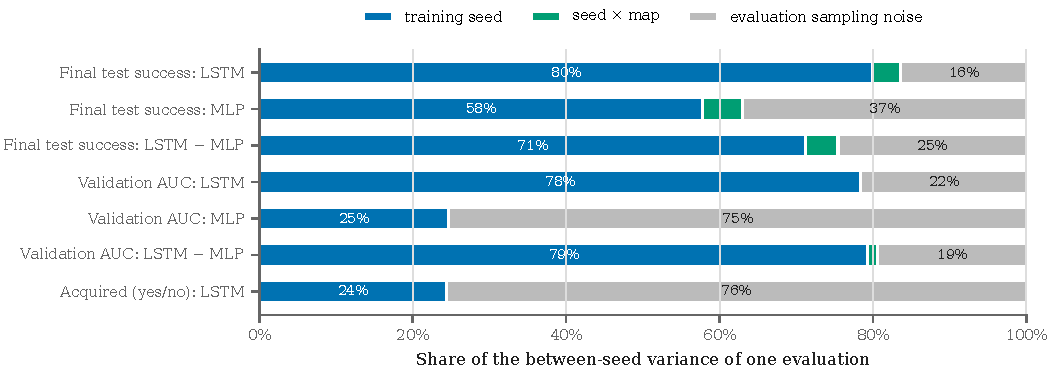
\includegraphics[width=\linewidth]{figures/fig_score_composition.pdf}
  \caption{Composition of the between-seed variance of a run's score from one evaluation, for
  each metric. Grey is the part due only to the randomness of evaluation. The MLP never
  acquires task B, so its acquisition verdict has no variance and is omitted.}
  \label{fig:composition}
\end{figure}

\subsection{How many seeds a claim needs}
\label{sec:results-seeds}

\Cref{fig:seeds} and \cref{tab:seeds} apply \cref{eq:dstudy} to the paired differences. With one
evaluation per run, as is common practice:
\begin{itemize}
  \item \textbf{Final test success.} Detecting a true gap of 20\pp{} takes 3 seeds, 10\pp{} takes
  11, and 5\pp{} takes 43. The pilot's three seeds could only have supported a gap of about
  20\pp{} or more. Three re-evaluations per run lower these numbers only slightly (43 to 36 for
  5\pp), because most of the per-seed variance is real seed variation, which more evaluations
  cannot remove.
  \item \textbf{Validation AUC} needs the fewest seeds (9 for 5\pp, 3 for 10\pp): averaging over
  the whole curve removes much of the noise. It measures speed and level together, however, so a
  gap in AUC is not a gap in final success.
  \item \textbf{The acquisition verdict} needs 93 seeds to detect a 10\pp{} difference in the
  fraction of seeds that acquire, and 369 for 5\pp. Here more evaluations do help (93 to 46 with
  three re-evaluations), because the verdict is mostly noise.
\end{itemize}
Claims about new maps rather than the fixed panel add the map term of \cref{eq:dstudy}. With 64
test maps that term alone is larger than a $\pm5$\pp{} target for the MLP, so no number of seeds
reaches that precision; for the paired gap the same target needs 178 seeds instead of 21. More
test maps, not more seeds, are what such claims require.

\begin{figure}[t]
  \centering
  \begin{minipage}[c]{0.49\linewidth}
    \centering
    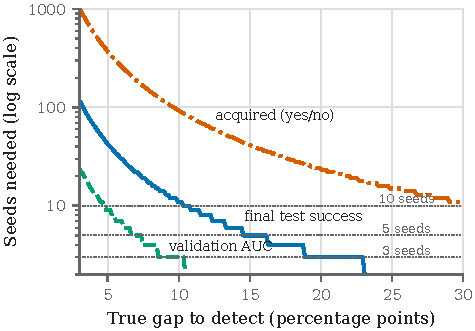
\includegraphics[width=\linewidth]{figures/fig_seeds_needed.pdf}
  \end{minipage}\hfill
  \begin{minipage}[c]{0.47\linewidth}
    \caption{Seeds needed for a paired two-sided test ($\alpha=0.05$, power 0.8) to detect a
    true gap between LSTM and MLP, with one evaluation per run, by metric. Dotted lines mark
    common seed counts. For the acquisition verdict the gap is a difference in the fraction of
    seeds that acquire the task.}
    \label{fig:seeds}
  \end{minipage}
\end{figure}

\begin{table}[t]
  \centering
  \caption{Seeds needed for the paired LSTM $-$ MLP comparison on the fixed test panel, with
  $n_r$ evaluations per run. Left: to detect a true gap $\delta$ ($\alpha=0.05$, power 0.8).
  Right: for a 95\% interval of half-width 5\pp{} around the mean gap.}
  \label{tab:seeds}
  \small
  \begin{tabular}{lcccccccc}
    \toprule
    & \multicolumn{2}{c}{$\delta=5$\pp} & \multicolumn{2}{c}{$\delta=10$\pp} &
      \multicolumn{2}{c}{$\delta=20$\pp} & \multicolumn{2}{c}{$\pm5$\pp{} interval} \\
    \cmidrule(lr){2-3}\cmidrule(lr){4-5}\cmidrule(lr){6-7}\cmidrule(lr){8-9}
    Metric & $n_r=1$ & $n_r=3$ & $n_r=1$ & $n_r=3$ & $n_r=1$ & $n_r=3$ & $n_r=1$ & $n_r=3$ \\
    \midrule
    Final test success & 43 & 36 & 11 & 9 & 3 & 3 & 21 & 18 \\
    Validation AUC & 9 & 8 & 3 & 2 & 2 & 2 & 5 & 4 \\
    Acquired (yes/no) & 369 & 183 & 93 & 46 & 24 & 12 & 181 & 90 \\
    \bottomrule
  \end{tabular}
\end{table}

\paragraph{Summary of Part I.}
On this task the LSTM's advantage over a memory-free MLP is large and robust: 25\pp, on 29 of 30
seeds. Measuring it reliably is easy for final success and AUC, and hard for the binary
acquisition verdict that learning curves are often summarised with. Most of the variation between
seeds in final success is real, so it is reduced by more seeds rather than more evaluations, and
claims beyond the test panel are limited by the number of maps.
